\section{Betrieb-, Infrastruktur- und Ausbildungskosten}
\label{s:Kosten}
In diesem Unterkapitel werden die Kostenstrukturen vorgestellt, wobei bei Betriebskosten wird auf die Kosten der Fluggesellschaft
eingegangen und bei Infrastruktur auf die Flughäfen, aufgrund abhängigen Kapitalkosten benötigt werden.

\subsection{Betriebskosten einer Fluggesellschaft}

Die Betriebskosten bei einer Flugzeugabfertigung werden auf Direct Operating Costs (DOC), und Indirect Operating Costs 
(IOC) geteilt, die werden auch Einzel- und Gemeinkosten genannt \cite{conrady2019luftverkehr}. 
DOC können einem bestimmten Flugzeug oder einer Strecke zugeordnet 
werden und können normalerweise als DOC pro Flugstunde, pro Kilometer, pro Passagierkilometer oder pro Blockstunde 
berechnet werden \cite{mensen2013handbuch}. 
Wobei IOC sind nicht direkt einem Flug zugewiesen, sondern für den gesamten Betrieb anfallen, wie z.B. zeitabhängige 
Instandhaltungskosten, Verwaltungskosten, Infrastrukturkosten \cite{mensen2013handbuch}. 

Nach der Beschäftigungsabhängigkeit werden die Kosten auf fixe und variable Kosten aufgeteilt. 
Fixe Kosten sind unabhängig von dem Betrieb (z.B. Kapitalkosten, Versicherung, Personalkosten), 
wo hingegen die variablen Kosten sich von der Beschäftigung ändern \cite{mensen2013handbuch}.

Die Struktur der Kosten einer Fluggesellschaft kann mit der Abbildung \ref{doc} veranschaulicht werden.

\begin{figure}[h]
	\centering
	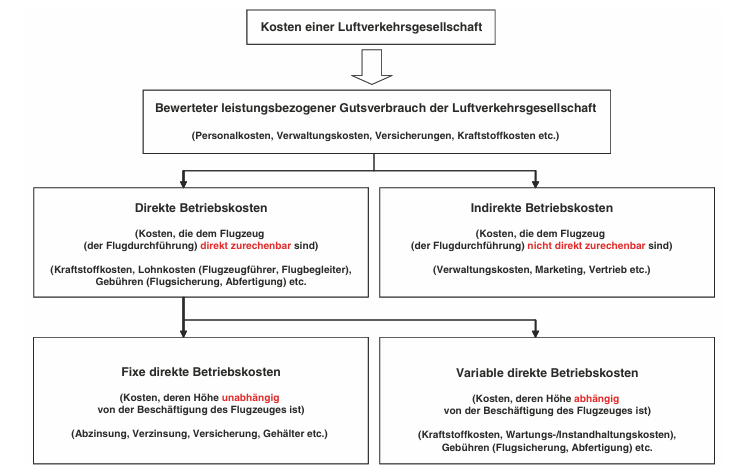
\includegraphics[width=0.9\linewidth]{Bilder/Systematik der DOC_Berechnung.png}
	\caption[DOC]{ \cite{mensen2013handbuch}}
	\label{doc}
\end{figure}

Betriebskosten sind von dem Flugzeugtyp abhängig, deswegen ist es wichtig vor der Anschaffung zu untersuchen, 
ob ein Flugzeug mit einem alternativen Antrieb rentabel ist. Die neuen Regularien für \ce{CO2}-Reduktion können einen Anreiz oder sogar 
eine Verpflichtung für die Fluggesellschaften schaffen, um die beste Lösung für eine Flotte zu finden. 
Mehr um politische Anreize gibt es im folgenden Unterkapitel \ref{s:Klimapolitische Maßnahmen}.
%
\textbf{Treibstoffkosten} sind ein erheblicher Teil der Betriebskosten. In den USA ein Drittel von allen Gesamtkosten (TOC) aller 
Fluggesellschaften sind die Kosten für Treibstoff und Öl, vergleichsweise (in Korrelation) beträgt die Abfertigung am Flughafen ein Sechstel 
\cite{conrady2019luftverkehr}. 
Im Jahr 2023 wurden etwa 92 Milliarden Gallonen Kraftstoff wurden durch der Luftfahrindustrie verbraucht und somit
war der Treibstoffrechnung fast 32 \% alles Betriebskosten in der Luftfahrt \cite{iata_industry_statistics_2024}.
Die jährlichen Steigerungen den Preisen für fossile Rohstoffe kann die nachhaltige Initiative fördern. \\
%Kesorinpreis im Jahr 2022 betrug USD 136/bbl, prognostiziert wird jedoch ...

"Betrachtet man den aktuellen Stand der kommerziellen Luftfahrt, so macht fossiles ATF den 
größten Teil des Energieverbrauchs im Luftverkehr aus, wobei Jet A und Jet A-1 überwiegend verwendet werden" %wo kommt das her?

%Technikkosten (Wartung, Reparatur, Instandhaltung MRO) - 
%es gibt unterschiedliche Typen von Wartung, die Kontrolle was am Vorfeld bei einem 
%Turnaround passiert ist die line maintenance (prüfung von Reifendruck und Ölständen), Flughafenentgelte und Handlingkosten: 
%Bodenabfertigung besteht aus Passagierabfertigung, Fracht-, Gepäckabfertigung und VorfelddiensteFlugzeugabfertigung ist direkte Kosten, 
%Passagierkosten indirekte Kosten, Kapital- und Abschreibungskosten \cite{conrady2019luftverkehr}. 
%Conrady bescheibt die Cockpit Crew als auch Cabin Crew, so Gehälter, Reisekosten, Schulungskosten. Es gibt jedoch nur wenige Arbeiten, 
%die die Ausbildungskosten erwähnen. Auch Handling Agents Kosten gibt es nicht viel Information zu finden. Es kann damit zurückgeführt werden, dass
%sind unabhängige von Fluggesellschaften Handling Agents für Abfertigung zuständig und nicht die Fluggesellschaften Kosten dafür übernehmen.

\textbf{Crewkosten} sind auch ein Bestandteil der direkten Betriebskosten. Zu einer Crew gehören Piloten und Kabine-Besatzung.
Nach Conrady \cite{conrady2019luftverkehr} bestehen die Besatzungskosten aus Gehälter, Reisekosten und Schulungskosten.
Es gibt jedoch nur wenige Arbeiten, die bei den Ausrechnungen Betriebskosten die Ausbildungskosten erwähnen. 

\subsection{Ausbildungskosten}

Die Schulungen sind ein wichtiger Teil der Ausbildung. 
%Über was geht in der annex
Nach ICAO Annex 6 muss das Schulungsprogramm muss eine Kompetenzschulung für alle installierten Geräte umfassen." (ICAO Annex 6 Teil 2)

\textbf{Wartungskosten} von einem Flugzeug fassen zusammen die Arbeitskosten für Beschäftigten und benötigten Materialien für die Wartung.
Außerdem werden die Kosten nach Wartung einer Zelle und den Triebwerken unterteilt \cite{wang2021research}. 
Meistens werden diese Komponente von unterschiedlichen
Unternehmen hergestellt (Quelle).
Am Vorfeld bei der Luftfahrzugabfertigung findet eine Line Maintenance statt, dabei wird der Reifendruck und Ölstände überprüft \cite{conrady2019luftverkehr}. 
Überdies gibt es eine Reihe anderen regelmäßigen Kontrollen.
Wartungskosten sind von Auslastung eines Flugzeugs, je mehr ein Flugzeug sich im Betrieb befindet, desto größere
Wartungskosten zu erwarten %schnellere Wartung man braucht, desto teurere Komponente man braucht.

Die Kurzstrecken-Flugzeuge sind mehr mit größerer Anzahl an Landungsgebühren und größere Treibstoffverbrauch verbunden sind, da 
der Start und die Landung sind die Treibstoff aufwendigste Prozesse im ganzen Flug.

Je nach Flotte sind die Ersparnisse möglich, wenn die Fluggesellschaften mehrere Flugzeuge vom gleichen Typ anschaffen \cite{conrady2019luftverkehr}. 
In diesem Fall weniger Schulungen für die Techniker notwendig.


%Eine Reihe anderen Kosten, die für die Arbeit vielleicht nicht relevant?: Flugsicherungsgebühren, Versicherungskosten (bleiben), 
%Servicekosten, Marketing- und Vertriebskosten, Kpsten der allgemeinen Verwaltung, 
In dieser Arbeit wird der Fokus auf die direkten Betriebskosten gelegt und die indirekten Betriebskosten, wie Kosten für 
allgemeine Verwaltung, Marketing- und Servicekosten, werden wegen geringere Relevanz nicht berücksichtigt.
%Diese werden aufgrund der Komplexität der Berechnungen und der begrenzten Verfügbarkeit von Daten nicht weiter betrachtet.


%Preis für Treibstoffversorgung für kurzfristige Perioden kann folgend berechnet werden \cite{iata_saf_procurement_2024}: nicht sicher, ob die Formel nehme
%PRA-Bewertung (Risikobewertung??? Durchschnitt der Vorperiode) + Logistikkosten + zusätzliche Gebühren + Lieferantenmarge

Kapitalkosten
Abschreibungskosten sind ein Teil der Kapitalkosten für das Flugzeug, die für den festgelegten Zeitraum, wo Flugzeug benutzt wird, verteilt.



%Conceptual_Design_and_Operating_Costs_Evaluation_of_a_19-seat_All-Electric_Aircraft_for_Regional_Aviation
"die Zins- und Abschreibungskosten sinken tendenziell bei hoher Tagesauslastung"
20 Prozent in Motorwartung verringert DOC um 4%


DMC are the maintenance costs caused directly by the aircraft; 
Wartung "line maintenance cost;
periodic maintenance cost;
workshop direct maintenance cost; and
overhaul cost."

\subsection{Infrastrukturkosten}

(Annex  Doc 1984 Teil 1 Chapter 13 Seite 141)
Bei konventionellen Kraftstoff kann die Logistik mit einem Schiff, Binnenschiff, Bahn, Lkw oder Pipeline durchgeführt. 
Diese Optionen haben große Auswirkungen auf die Kapitalkosten eines Flughafens und müssen sorgfältig berechnet werden. 
eine von spezialen Anforderungen bei Planung von Flughafeninfrastruktur "Minimierung der Belegungszeiten am Flugzeuggate; 
die erforderlichen Kraftstoffdurchflussraten sind ein Faktor bei der Wahl des einzusetzenden Betankungssystems"